\section{Inverse Problems} 
\label{sec:inverse}
\begin{shaded}
\noindent In this section, I will provide a general summary of inverse problems, with particular attention toward those that are posed and solved in the subsequent chapters of this thesis. 
Several textbooks discuss inverse problems and their solutions. 
In writing this section, I have made use of the textbooks by \citet{basuchaplin2017}, \citet{kirsch2011introduction} and \citet{neto2012introduction}. 
Additionally, I have found the reviews by \citet{tenorio2001statistical}, \citet{GoughThompson1991}, and \citet{2018ASSP...49...75R} helpful. 
\end{shaded}

So far we have concerned ourselves with discussions of \emph{forward problems}. 
These can be thought of as problems where we have a theory, we input some initial conditions, and we compute the result deterministically. 
The two topics of the previous chapters have been the theory of stellar evolution and the theory of stellar pulsation. 
In the case of evolution, we supplied the initial conditions (mass, initial composition, mixing length parameter, etc.), and then applied the theory to simulate what such a star would be like at each given time in the future. 
%At each time step, we have observable quantities, such as the stellar luminosity, as well as ``unobservable'' quantities, such as the mixture of elements in the core. 
In the case of pulsation, we supplied a static stellar structure, and then applied the theory to calculate the corresponding frequencies of oscillation. 
Now we wish to go in the opposite direction (see Figure~\ref{fig:forward-inverse}). 

\begin{figure}
    \centering
    \begin{tikzpicture}[
        ->, 
        thick, 
        main node/.style={
            circle, 
            draw,
            minimum height=5em,
        },
        node distance=10em, 
        auto,
        pil/.style={
           thick,
           shorten <=2pt,
           shorten >=2pt
        }
    ]
    \node[main node, fill=blue!20!white] (model) {Model};
    \node[main node, right=of model, fill=orange!20!white] (data) {Data}
        %\draw[decoration={markings, mark=at position 1 with {\arrow[ultra thick]{>}}}, postaction={decorate}, bend left=30] %(model) to (data) 
        %node[above] {Forward Problem} (model);
        edge[pil, <-, bend right=30] node[above, yshift=0.1cm] {\sffamily\small{Forward Problem}} (model)
        edge[pil, ->, bend left=30] node[below, yshift=-0.1cm] {\sffamily\small{Inverse Problem}} (model);
\end{tikzpicture}

    \caption[Forward and Inverse Problems]{A schematic for the relationship between forward and inverse problems. 
            In the forward problem, we use the theory or a model to generate data, such as the types of information that could be observed about a system. 
            In the inverse problem, we seek to reconstruct all the possibilities that are consistent with that observed data. 
        \label{fig:forward-inverse}}
\end{figure}

\epigraph{``\emph{The cause is hidden, but the result is known.}''}{--- Ovid\\\emph{Metamorphoses} (\citeyear{ovid})}


In the case of evolution, given the observation of a star (e.g., its luminosity, or pulsation data), we wish to determine its overall properties (e.g., mass, radius, age) and evolutionary history (initial composition and so on) using the theory of evolution. 
In the case of pulsation, given the observed oscillation frequencies, we wish to determine the stellar structure that supports those oscillations using the theory of stellar pulsation. 
These are the inverse problems of asteroseismology that form this thesis. 

%Given the observations of a star, we want to determine its evolutionary initial conditions and its internal structure. 


%


The difficulty in solving these problems comes in part from the fact that they are \emph{ill-posed}. 
%What does it mean for a problem to be ill-posed? 
At the beginning of the 20th century, the French mathematician \mycitet{hadamard} gave his definition for what constitutes a well-posed problem. 
Hadamard believed that problems worth consideration should have the properties that
\begin{enumerate}
    \item a solution exists (existence), 
    \item the solution is unique (uniqueness), and 
    \item the solution changes continuously with changes to the input (stability). 
\end{enumerate}
A problem that fails to meet one or more of these criteria is then said to be ill-posed. 

\epigraph{``\emph{The respect for Hadamard was so great that incorrectly posed problems were \hphantom{``}considered `taboo' for generations of mathematicians, until comparatively recently \hphantom{``}it became clear that there are a number of quite meaningful problems, the so-called \hphantom{``}`inverse problems,' which are nearly always unstable with respect to fluctuations \hphantom{``}of input data.}''}{--- H.\ Allison\\\emph{Inverse Unstable Problems and Some of Their Applications} (\citeyear{allison1979inverse})}

An example of a well-posed problem is: given the formula for a line and some coordinates, calculate the corresponding points on the line. 
The inverse of this problem---calculating the formula of a line given points belonging to it---also happens to be well-posed. 
Suppose however that we only have one point. 
Then the uniqueness condition is not satisfied, as infinitely many lines pass through that point. 
Suppose instead that we have multiple points, but one of the points does not actually belong to the line. 
Then the existence condition is not satisfied, as no one line passes through all the points. 

One of the most famous inverse problems is the question from mathematician Mark Kac: ``Can One Hear the Shape of a Drum?'' \citep{10.2307/2313748}. 
In a response article entitled ``You Can't Hear the Shape of a Drum,'' \citet{10.2307/29775597} produced two different drums with the same eigenfrequencies. 
The solution to the problem therefore lacks uniqueness, and so it is ill-posed. 

The solutions to physical inverse problems often lack uniqueness. 
At a basic level, measurements are nearly always uncertain, and therefore the solution is uncertain. 
Less obvious however is that two distinct sets of initial conditions can often lead to the same observables (i.e., the forward function is non-injective, see Figure~\ref{fig:non-injective}). 
This is sometimes referred to as degeneracy. 
The evolution inverse problem has the additional issue that there are observations of stars (the Sun is an example) that cannot yet be fully reproduced by any evolutionary model (i.e., the forward function is non-surjective, see again Figure~\ref{fig:non-injective}). 
This is one reason why we separate the two inverse problems, and use the solution from the evolution inversion as the starting point for the structure inversion. 

\begin{figure} 
    \centering 
    \begin{tikzpicture}[
        ele/.style={
            %fill=black,
            %circle,
            minimum width=.8pt,
            inner sep=1pt},
            every fit/.style={ellipse,draw,inner sep=-2pt}
        ]
    \node[ele] (a1) at (0,4) {$1$};
    \node[ele] (a2) at (0,3) {$2$};
    \node[ele] (a3) at (0,2) {$3$};
    \node[ele] (a4) at (0,1) {$4$};
    
    \node[ele] (b1) at (4,4) {$a$};
    \node[ele] (b2) at (4,3) {$b$};
    \node[ele] (b3) at (4,2) {$c$};
    \node[ele] (b4) at (4,1) {$d$};
    
    \node[draw,fit= (a1) (a2) (a3) (a4),minimum width=2cm, thick, fill=orange!20!white] (leftoval) {} ;
    \node[draw,fit= (b1) (b2) (b3) (b4),minimum width=2cm, thick, fill=blue!20!white] (rightoval) {};
    
    \node[above of=leftoval, yshift=1.75cm] {\sffamily Models};
    \node[above of=rightoval, yshift=1.75cm] {\sffamily Data};
    
    \draw[->,thick,shorten <=5pt,shorten >=5pt] (a1) -- (b1);
    \draw[->,thick,shorten <=5pt,shorten >=5pt] (a2) -- (b2);
    \draw[->,thick,shorten <=5pt,shorten >=5pt] (a3) -- (b3);
    \draw[->,thick,shorten <=5pt,shorten >=5pt] (a4) -- (b3);
    %\draw[->,thick,shorten <=2pt,shorten >=2] (a4) -- (b3);
    \node[ele] (a1) at (0,4) {$1$};
    \node[ele] (a2) at (0,3) {$2$};
    \node[ele] (a3) at (0,2) {$3$};
    \node[ele] (a4) at (0,1) {$4$};
    
    \node[ele] (b1) at (4,4) {$a$};
    \node[ele] (b2) at (4,3) {$b$};
    \node[ele] (b3) at (4,2) {$c$};
    \node[ele] (b4) at (4,1) {$d$};
\end{tikzpicture}

 
    \caption[Non-injective and non-surjective functions]{Physical systems are often \emph{non-injective} in the sense that two systems may have different internal conditions but the same external observables. 
    Here models $3$ and $4$ share the same set of observables $c$. 
    This system is also \emph{non-surjective} because the fourth set of observations is not produced by any model. 
        \label{fig:non-injective}}
\end{figure}

The word ``inverse'' is especially appropriate because inverse problems can often be stated as finding the inverse of a forward function, operator, or matrix. 
For example, if we have a model $M$ that takes initial conditions $x$ and produces data ${y=M(x)}$, then the inverse problem is to determine ${x=M^{-1}(y)}$ from observations of $y$. 
This is where the condition of stability often runs into problems. 

As an example, consider a simple theory defined by the following linear system of equations:
\begin{alignat}{3}
    &x_1 + x_2& &= y_1 \\
    &x_1 + (1+\epsilon)x_2& &= y_2
\end{alignat}
where $\epsilon$ is an arbitrarily small number. %, say $\epsilon=10^{-10}$. 
The values $y_1$ and $y_2$ are then observed in nature, each coming up to be ${y_1=y_2=2}$. 
We now seek the ``initial conditions'' ${\mathbf{x} \equiv (x_1,x_2)}$ to explain this observation. 
The solution is clearly ${\mathbf{x}=(2,0)}$. 
Now consider that $y_2$ was instead measured to be ${2+\epsilon}$. 
The solution then changes to ${\mathbf{x}=(1,1)}$. 
Recall however that $\epsilon$ was chosen to be arbitrarily small. 
Thus, an arbitrarily small change to the measurement has completely changed the solution. 
To be even more concrete, if we let ${\epsilon=10^{-10}}$ and modify $y_2$ to be, say, ${2+10^{-5}}$, then we obtain ${\mathbf{x}\simeq(-99998, 10000)}$. 
The system is unstable. 

In matrix notation, this system corresponds to
\begin{equation}
    \mathbf{M}\mathbf{x}
    =
    \mathbf{y},
    \qquad
    \mathbf{M}
    =
    \begin{bmatrix}
        1 & 1 \\
        1 & 1+\epsilon 
    \end{bmatrix}. \iffalse,
    \qquad
    %\qquad\text{and}\qquad
    \mathbf{y}
    =
    \begin{bmatrix}
        2\\2
    \end{bmatrix}.
    \fi
\end{equation}
Here our model is the nearly singular matrix $\mathbf{M}$, we have observed the data $\mathbf{y}$, and we've sought the initial conditions ${\mathbf{x}=\mathbf{M}^{-1}\mathbf{y}}$. 
%However, $\mathbf{M}$ is very nearly singular. %, and so as we've seen, the solution is unstable with respect to small changes in the input. 
When the condition number ${\kappa(\mathbf{M})=||\mathbf{M}||\;||\mathbf{M}^{-1}||}$ is large, the problem is said to be ill-conditioned. 
When ${\kappa = \infty}$, the problem is ill-posed. 
For this particular system, 
\begin{equation}
    \lim_{\epsilon\to 0} \kappa(\mathbf{M}) = \infty.
\end{equation}

The kernel functions that we derived in the previous section are nearly linearly dependent across the different modes, and so the structure inversion problem is ill-conditioned. 
As we will see later, such problems are generally dealt with by enforcing stability or regularity conditions, i.e., regularization \citep[e.g.,][]{tikhonov1977solutions, tenorio2001statistical}. 

%Solutions to the helioseismic and geologic inversion problems have provided detailed pictures of the Sun and the Earth. 


\subsection{Evolution Inversions} 

With the equations of Section~\ref{sec:evolution} and some chosen initial conditions, we can simulate the life of a star, and at each step of the way, determine what observations of that star would yield. 
Thus we have a forward model $M$ which is parameterized by initial conditions $\mathbf{x}$ and time $\tau$, and yields data $\mathbf{y}$:
\begin{align}
    M(\mathbf{x}, \tau)
    &=
    \mathbf{y}
    \\
    \mathbf{x}
    &=
    [M,Y_0,Z_0,\alpha_{\text{MLT}}, \ldots]%,\alpha_{\text{MLT}},\alpha_{\text{ov}},D]
    \\
    \mathbf{y}
    &=
    [L, T_{\text{eff}}, \text{[Fe/H]}, \boldsymbol{\nu}, \ldots].
\end{align}
We now seek to interpret observations of a star in the context of the theory of stellar evolution. 
In other words, we seek the inverse function:
\begin{equation}
    M^{-1}(\mathbf{y})
    =
    [\mathbf{x}, \tau].
\end{equation}
Of course, we can also seek a function that outputs additional quantities at the present age, such as the radius if it has not been observed. 
There are several approaches that have been taken to solve this problem, which I will now review. 

\subsubsection*{Scaling Relations}
\label{sec:scaling}
A simple approach to estimate stellar properties is to ``scale'' them from solar values using the equations of stellar structure and pulsation. 
While such an approach does not solve the full evolution inversion problem, it shares a common goal of estimating (a more limited set of) properties such as the stellar mass. 
%However, scaling relations are similar to evolution inversions in that the end result of each is stellar parameter estimations, albeit a more limited set. 
%are the solar scaling relations. 
%Scaling relations take the equations of stellar physics and ``scale'' them from the solar values to the observed values of other stars. 

A simple example comes from the Stefan-Boltzmann law (Equation~\ref{eq:stefan-boltzmann}). 
Replacing this equation with ratios with respect to the solar values, we may obtain 
\begin{equation}
    \frac{R_\ast}{R_\odot}
    =
    \left(
        \frac{L_\ast}{L_\odot}
    \right)^{-2}
    \left(
        \frac{T_{\text{eff},\ast}}{T_{\text{eff},\odot}}
    \right)^4
\end{equation}
from which we can estimate an unknown stellar radius $R_\ast$ from a measured stellar luminosity $L_\ast$ and effective temperature $T_{\text{eff},\ast}$. 
In principle, this relation works; in practice, the luminosities of most stars are unknown, and effective temperatures are measured rather imprecisely (${\gtrapprox 50}$~K uncertainty). 

The same kind of manipulation can be used on the asymptotic equations of stellar pulsation to obtain stellar masses and radii. 
From manipulation of Equations~(\ref{eq:numax}) and (\ref{eq:Dnu}) we find \citep[e.g.,][]{1995A&A...293...87K}:
\begin{align}
    \frac{R_\ast}{R_\odot}
    &=
    \left(
        \frac{\nu_{\max,\ast}}{\nu_{\max,\odot}}
    \right)
    \left(
        \frac{\Delta\nu_\ast}{\Delta\nu_\odot}
    \right)^{-2}
    \left(
        \frac{T_{\text{eff},\ast}}{T_{\text{eff},\odot}}
    \right)^\frac{1}{2}
    \\
    \frac{M_\ast}{M_\odot}
    &=
    \left(
        \frac{\nu_{\max,\ast}}{\nu_{\max,\odot}}
    \right)^3
    \left(
        \frac{\Delta\nu_\ast}{\Delta\nu_\odot}
    \right)^{-4}
    \left(
        \frac{T_{\text{eff},\ast}}{T_{\text{eff},\odot}}
    \right)^\frac{3}{2}
\end{align}
which hold to decent approximation. 
\citet{2017ApJ...843...11V} recently pointed out that the $\nu_{\max}$ scaling relation can be improved by including a term for the mean molecular weight. 

As stars evolve into giants, the assumption of homology breaks down more and more, leading to systematic errors as high as $15\%$ \citep[e.g.,][]{2016ApJ...832..121G}. 
By comparison of theoretical red giant model mode frequencies with those given by the scaling relations, \citet{2016MNRAS.460.4277G, 2017MNRAS.470.2069G} developed metallicity-dependent and mass-dependent corrections to the $\Delta\nu$ scaling relation. 

These scaling relations do not tell us about the age or evolution of the star. 
We saw previously that the small frequency separation probes the sound speed gradient, which is then an indicator on the main sequence of the conditions in the core, and therefore main-sequence age. 
The so-called C--D diagram shows the core-hydrogen abundance and stellar mass as a function of the frequency separations (\citealt{1984srps.conf...11C}, see also Figure~\ref{fig:jcd}). 
%Under assumption of a solar-calibrated mixing length and solar abundances
If all stars had the solar abundances and solar mixing length, it would suffice to look up their mass and core-hydrogen abundance in this diagram. 
Since they do not, a more sophisticated approach is required. 

%\iffalse
%\afterpage{
%\begin{landscape}
\begin{figure}
    \centering
    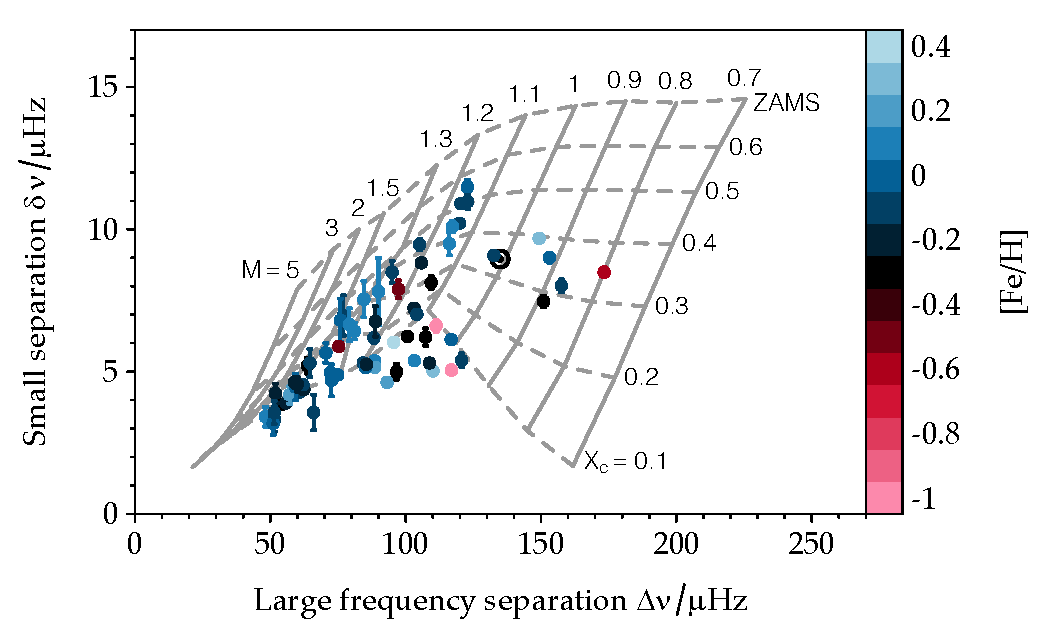
\includegraphics[width=\textwidth]{figs/pulse/CD.pdf}%{../LEGACY/Bellinger_E_fig1.pdf}
    \caption[C--D Diagram]{The C--D diagram. 
    The small frequency separation is a proxy for core hydrogen abundance ($X_c$, dashed lines) through the sound speed gradient, and the large frequency separation is a proxy for stellar mass ($M$, solid lines) through the mean density. 
    The gray lines are evolutionary simulations varied in their initial mass and evolved along the main sequence. 
    The frequencies of the models have been calculated using GYRE \citep{2013MNRAS.435.3406T}. 
    Stars with ${M \gtrapprox 1.8\;M_{\odot}}$ do not have convective envelopes on the main sequence and are therefore not theoretically predicted to harbor solar-like oscillations. 
    %C-D diagram showing small frequency separations against large frequency separations with [Fe/H] indicated by color for 52 main-sequence \emph{Kepler} LEGACY stars overplotted on top of evolutionary models varied in mass with solar-calibrated mixing length and abundances generated using MESA with frequencies calculated using GYRE \citep{2013MNRAS.435.3406T}. 
    The points are LEGACY stars observed by \emph{Kepler}, colored by their metallicity \citep{2017ApJ...835..172L}. 
    Many of the stars fall off the diagram, thus illustrating its limitations as a look-up table for stellar properties. 
    %Since they do not, a more sophisticated approach is required; here we employ the method introduced in \citealt{2016apj...830...31b} (Chapter~\ref{chap:ML}) for this task.
    \emph{Figure adapted from \citealt{2017EPJWC.16005003B}.} 
    \label{fig:jcd}} 
    %\caption[The C-D Diagram]{}
\end{figure}
%\end{landscape}
%}
%\begin{figure}
    %\contcaption{The C-D diagram. 
    %The small frequency separation is a proxy for core hydrogen abundance X_c, and the large frequency separation is a proxy for stellar mass. 
    %The gray lines are 
    %C-D diagram showing small frequency separations against large frequency separations with [Fe/H] indicated by color for 52 main-sequence \emph{Kepler} LEGACY stars overplotted on top of evolutionary models varied in mass with solar-calibrated mixing length and abundances generated using MESA with frequencies calculated using GYRE \citep{2013MNRAS.435.3406T}. 
    %If all stars had the solar abundances and solar mixing length, it would suffice to look up their mass and core-hydrogen abundance in this diagram. 
    %Since they do not, a more sophisticated approach is required; here we employ the method introduced in \citealt{2016apj...830...31b} (Chapter~\ref{chap:ML}) for this task.
    %\emph{Figure adapted from \citet{2017EPJWC.16005003B}.} 
    %\label{fig:jcd}} 
%\end{figure}
%\fi
%For this we need a more sophisticated approach. 
%, its initial or current chemical composition, 
%These relations hold to decent approximation for main-sequence stars of solar metallicity. 

%testing scaling relations \citep{2011ApJ...743..143H}

\iffalse
From the modeling point of view, the scaling relations are used to determine $\nu_{\max}$ of a stellar model, as it cannot currently be predicted theoretically. 
We remain in want of a proper treatment of convection in stars, and so it is not currently possible to determine mode amplitudes and lifetimes. 
Following the analysis by \citet{2015A&A...583A..74J}, \citet{2017ApJ...843...11V} have recently argued that a term for the mean molecular weight $\mu$ should be added to the theoretical calculation of $\nu_{\max}$, as 
\begin{equation}
    \nu_{\max} \propto \nu_{\text{ac}} \propto g\sqrt{\frac{\mu}{T_{\text{eff}}}}%{\sqrt{T_{\text{eff}}}}
\end{equation}
and therefore
\begin{equation}
    \frac{\nu_{\max,\ast}}{\nu_{\max,\odot}}
    =
    \left(
        \frac{M_\ast}{M_\odot}
    \right)
    \left(
        \frac{R_\ast}{R_\odot}
    \right)^{-2}
    \left(
        \frac{T_{\text{eff},\ast}}{T_{\text{eff},\odot}}
    \right)^{-\frac{1}{2}}
    \left(
        \frac{\mu_\ast}{\mu_\odot}
    \right)^{\frac{1}{2}}.
\end{equation}
\fi

%In asteroseismology, there are two common scaling relations: one from $\nu_\max$ and one from $\Delta\nu$. 

%There are two 
%From an observed power excess, we may transform $\nu_\max$ into the mean density of 



\subsubsection*{Repeated Forward Modelling} 
A more involved approach to determining the properties of stars is through repeated forward modelling. 
Such an approach can also be applied to non-solar-like stars (e.g., evolved stars) where homology relations break down. 
%This can be achieved through either \emph{grid-based modelling} or \emph{iterative optimization}. 
These methods still make no attempt to determine the function $M^{-1}$. 
Though there are variations, they instead try to optimize the result of the forward operator against the observations: 
\begin{equation}
    [\hat{\mathbf x}, \hat\tau]
    =
    \underset{[\mathbf x, \tau]}{\arg\min}\; \left[
        M(\mathbf x, \tau)
        -
        \mathbf y
    \right]^T
    %\cdot
    \boldsymbol{\Sigma}_{\mathbf y}^{-1}
    \left[
        M(\mathbf x, \tau)
        -
        \mathbf y
    \right]
\end{equation}
where $\hat\cdot$ means the optimal $\cdot$, and $\boldsymbol\Sigma_{\mathbf y}$ is the covariance matrix for the observations. 
%\newpage
%\noindent 
There are several drawbacks with this approach: 
\begin{description}
    \setlength{\itemindent}{0pt}
    \item[Speed.] This approach can be prohibitively slow, especially if new models need to be computed for each input, or if multiple input parameters are being optimized. 
    This is often dealt with by applying additional assumptions to simplify the problem. 
    For example, the mixing length parameter can be kept fixed to the solar-calibrated value \citep[e.g.,][]{2015MNRAS.452.2127S,2017ApJ...835..173S}. 
    Another simplification is to calculate the initial helium abundance from the initial metallicity by assuming a galactic chemical evolution law \citep[e.g.,][]{2015MNRAS.452.2127S, 2017ApJ...835..173S}. 
    This is usually achieved by fitting a line through to two points: the primordial helium abundance from models of Big Bang nucleosynthesis $[Y_p=0.2463,Z_p=0]$ \citep[e.g.,][]{2014JCAP...10..050C} and the calibrated initial solar mixture, e.g., ${[Y_{0,\odot}=0.273,Z_{0,\odot}=0.019]}$, so ${\Delta Y/\Delta Z \simeq 1.4}$. 
    %, such as that all stars can be modeled using the solar-calibrated mixing length, or that the initial helium abundance can be found by interpolating between the primordial helium abundance and the solar values. 
    The optimization is then performed over a limited set of input parameters (e.g., ${[M,Z_0]}$) and potentially on a pre-computed grid of models as well. 
    However, the end result then has (typically unpropagated) systematic errors. 
    %The end result then has unpropagated systematic errors from these assumptions. 
    
    \item[Local Minima.] Commonly, iterative numerical optimization algorithms such as
    %Levenberg--Marquardt \citep{10.2307/43633451,10.2307/2098941}
    \citeauthor{10.2307/43633451}--\citeauthor{10.2307/2098941} (\citeyear{10.2307/43633451,10.2307/2098941})
    and %Nelder--Mead 
    \mycitet{nelder1965simplex}
    %\citetalias{nelder1965simplex} (\citeyear{nelder1963simplex})
    are applied for this task \citep[e.g.,][]{2014A&A...569A..21L, 2015A&A...582A..25A}. 
    These approaches can have difficulty finding global minima of the solution. 
    %This approach can have difficulties with local minima. 
    %Commonly, optimization algorithms such as Levenberg--Marquardt and Nelder--Mead are applied for this task, which are known to ``get stuck'' \citep[e.g.,][]{2014A&A...569A..21L, 2015A&A...582A..25A}. 
    %Approaches such as those based on MCMC can avoid this pitfall, but again run into the first problem. 
    %The most common approach is the 
    %and techniques to avoid this issue then run into the first problem again. 
    
    %\item[Complexity.] 
    There are also no currently known theoretical bounds on the complexity of a Nelder-Mead search \citep{singer1999complexity}. 
    It is however known that this algorithm scales poorly to high dimensions \citep[e.g.,][]{Chen2015}. 
    
    \item[Redundancy.] This approach implicitly assumes that each bit of observable information provides a fully independent constraint to the stellar model, and weights each observation only by its uncertainty. 
    In reality, the observations have some degree of redundancy with respect to the aspects of the model that they constrain (\mycitealt{2017apj...839..116a}, see also Chapter~\ref{chap:statistical}). 
    Matching such an aspect of the model is then arbitrarily upweighted. 
    Some practitioners deal with this problem by applying \emph{ad hoc} weightings \citep[e.g.,][]{2013apjs..208....4p}. 
\end{description}
We therefore seek an approach that naturally avoids these problems. 

\subsubsection*{Random Forest Regression} 
In recent years, machine learning techniques have become increasingly popular for solving inverse problems \citep[e.g.,][]{rosasco2005learning, fai2017inner, 2017InvPr..33l4007A}. 
%Such techniques have been especially applied in medical informatics. 
Some applications include automatic photograph coloration \citep{larsson2016learning}, image reconstruction \citep[e.g.,][]{2017arXiv170300555S}, and medical imaging \citep[e.g.,][]{prato2008inverse, jin2017deep}. 
In fact, supervised learning itself can be viewed as an inverse problem \citep{vito2005learning}. 

In Chapter~\ref{chap:ML} we propose a solution to the evolution inversion problem based on machine learning. 
In particular, we use the variant of random forest regression \citep{breiman2001random} known as extremely randomized trees \citep{geurts2006extremely} to learn the function $M^{-1}$ from a dense grid of evolutionary simulations. 
%In particular, . %according to the set of observations that are available 
%We choose an ensemble-based approach---random forests---to deal with the degeneracy of the problem. 
Ensemble tree-based algorithms are known to be quick to train (especially because the task is `embarrassingly' parallelizable), quick to predict (when the number of trees is not very large), and to have very good predictive performance \citep[e.g.,][]{Caruana:2006:ECS:1143844.1143865}. %even when the features are redundant or uninformative. 
Furthermore, the bootstrap aggregation (``bagging'') that is performed helps with problem degeneracy and dimensionality \citep[e.g.,][]{Skurichina2002}. 
Random forests can suffer from reduced performance if the number of redundant variables is large \citep{louppe2014understanding}, however there are strategies to deal with this drawback \citep{tuv2009feature}. 

\citet[][]{louppe2014understanding} derived the worst-case time complexity of training extremely randomized trees to be ${\mathcal{O}(MKN^2)}$, where $M$ is the number of trees, $N$ is the number of samples, and $K$ is the number of features that is randomly drawn at each node. 
In Chapter~\ref{chap:ML}, we cross-validate $M$ and find satisfactory performance at ${M=256}$. 
The parameter $K$ varies between $2$ and $9$, depending on the types of observations available for a given star. 
%and $N$ and find satisfactory performance at $M=256$ and $N=$



%\citet{prato2008inverse} used machine learning to solve inverse problems related to translating functional magnetic resonance imaging data into measures of brain activity. 


To obtain the posterior distribution of solutions for an observed star with measurement uncertainties, we pass random instances of the observations perturbed by their uncertainties through the trained network. 
%\paragraph*{Propagating Uncertainties} 
%\noindent When propagating the empirical uncertainties, 
We have to choose how many random instances that we will use. 
This number should be chosen such that the sample distribution converges to a reasonable degree to the population distribution. 
A useful way to quantify the differences in distributions is the Kullback-Leibler (KL) divergence, also known as relative entropy: 
\begin{equation} \label{eq:KL}
    D_{\text{KL}} (P||Q) = \int_{-\infty}^\infty p(x) \log \frac{p(x)}{q(x)} \;\text{d}x
\end{equation}
where $P$ and $Q$ are two continuous random variables and $p$ and $q$ are their respective densities \citep{10.2307/2236703}. 
A low relative entropy indicates similarity. %of the distributions. %that the distributions are quite similar, if not identical. 

We seek to determine how many random samples we need to generate in order for our posterior distributions to converge to a reasonable degree to their actual distributions. 
A proxy for this would be to determine the KL divergence between the normal distribution and sample normal distributions of varying sizes. 
Figure \ref{fig:kl} shows an example of a standard normal distribution $\psi$ and sample normal densities with different sample sizes. 
The figure furthermore shows the KL divergence of these sample normal distributions as a function of sample size, averaged over $1,000$ random trials. 
The distribution converges around $10,000$ samples. 
Thus, we propagate $10,000$ random instances of the measurement uncertainty through the random forest. 
%which gives the relative entropy between two probability distributions . 
Applying the technique fleshed out in detail in Chapter~\ref{chap:ML} to $94$ stars observed by \emph{Kepler}, we find the estimates shown in Figure~\ref{fig:posterior-cdf}. 

\begin{figure}
    \centering
    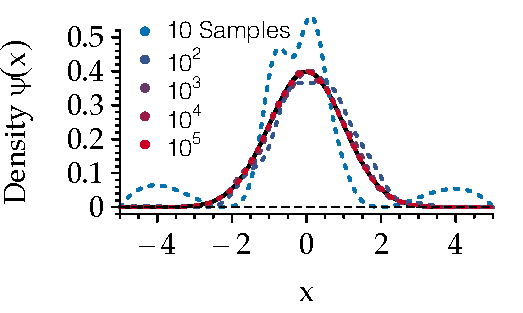
\includegraphics[width=0.5\textwidth]{figs/evol/norm.pdf}%
    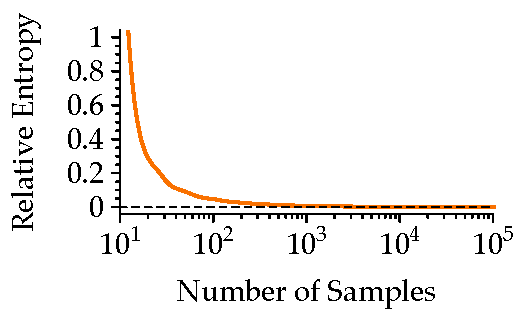
\includegraphics[width=0.5\textwidth]{figs/evol/KL.pdf}
    \caption[Relative entropy of sample normal distributions]{Left: Normal density distribution (black line) and example sample normal distributions for various sample sizes (dashed lines). 
    Right: Average divergence of sample normal distributions from the standard normal distribution as a function of sample size. 
    \label{fig:kl}}
\end{figure}

\begin{figure}
    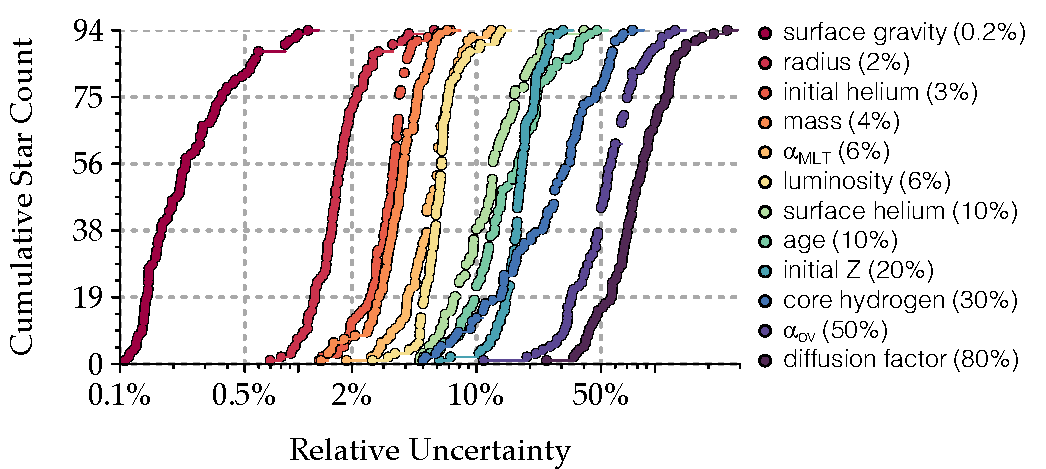
\includegraphics[width=\textwidth]{figs/pulse/cdf.pdf}
    \caption[Relative uncertainties in estimated stellar parameters]{Cumulative distribution functions showing the relative uncertainties in estimated stellar parameters for $94$ main-sequence stars. 
    Each type of measurement is sorted by uncertainty. 
    The numbers in parentheses in the legend give the median uncertainty. 
    \emph{Figure adapted from \citealt{2017EPJWC.16005003B}.}
    \label{fig:posterior-cdf}}
\end{figure}


\subsection{Structure Inversions} 
By solving the evolution inverse problem, we can obtain an evolutionary model for a given observed star. 
However, regardless of the technique used, the mode frequencies of best-fitting models generally fail to match one or more mode frequencies of the star---even after correcting surface effects. 
This implies that the structure of the star differs from the structure of the model. 
This is the starting point for the structure inversion problem. 
We seek to invert Equation~(\ref{eq:forward-surf}) to infer ${f_1(r)}$ from observed mode frequencies, for some choice of $f_1$, by deducing the difference in $f_1$ between the best-fitting model and the star. 
This problem is difficult for multiple reasons: 
\begin{description}
    \setlength{\itemindent}{0px}
    \item[Degeneracy.] As the kernels reveal, a modification to the structure anywhere in a stellar model may cause several or all of its pulsation modes to shift in their frequency of oscillation, and each frequency may shift in a different way. 
    Modifications to different locations in the stellar interior may also cause the same change to the frequency of a mode. 
    
    Furthermore, the mode frequencies are a function of multiple structural quantities. 
    When trying to infer $f_1$, we must ensure that the results are not unduly influenced by $f_2$. 
    With the present quality of asteroseismic data, this restricts us to kernel pairs with ${f_2=Y}$ (recall Section~\ref{sec:kernels}). 
    
    \item[Information Content.] 
    Whereas we are trying to measure a continuous function, which in principle may contain infinite information, we have only a finite set of mode frequencies with which to do it. 
    
    Furthermore, we will only be able to form well-localized averaging kernels in regions where a sufficient number of lower turning points are situated (recall Figure~\ref{fig:rays}). 
    This rules out some inversion methods. 
    
    %\item[Stability.] 
    \item[Stability.]  The kernel functions are nearly linearly dependent, and so the problem is ill-conditioned. 
    Even if the measurements of the mode frequencies were certain, an exact fit to mode frequencies yields highly oscillatory, non-physical solutions \citep[see, e.g.,][]{1990MNRAS.244..542D}. 
    %Furthermore, the measurements of the mode frequencies are uncertain. 
    
    \item[Surface Effects.] All of the modes are sensitive to the outermost layers of the star, where our assumptions break down (recall Sections~\ref{sec:evolution} and \ref{sec:pulsation}). 
    Thus, we must take special care to suppress surface effects. 
    However, there may be additional surface effects that the present treatment do not suppress. 
    The treatment of the surface term may furthermore erroneously subtract off more than just surface effects. 
    
    \item[Uniqueness.] The solutions are not unique. 
    From any solution to the inverse problem, a different solution can be generated %by considering the combination of regions to which the observed modes are not sensitive 
    (see \citealt{GoughThompson1991} for a discussion). 
\end{description}
As discussed in the first section, inversion of asteroseismic data presents some novel challenges over helioseismic inversions \citep[e.g.,][]{2014aste.book...87B}. 
Unlike in helioseismology, in which the solar mass and radius are known to high precision, the masses and radii of solar-type oscillating stars are generally uncertain by at least a percent \citep[see e.g.,][see also Figure~\ref{fig:posterior-cdf}]{2013MNRAS.433.1262W,2015MNRAS.452.2127S,2016apj...830...31b}. 
Although seemingly small, such uncertainties in stellar mass and radius are generally about two orders of magnitude greater than the uncertainties in oscillation mode frequencies. 
The number of observed oscillation modes is also much smaller, and the inner radii at which these modes turn around is much more limited as well. 

The most `obvious' way to invert Equation~(\ref{eq:forward-surf}) would be via a least squares fit to the entire unknown profile. 
That is: replace the functions to be estimated by linear basis functions \citep[e.g., cubic B-splines,][]{de1972calculating}, and then select the coefficients of the basis functions such that the residuals are minimized \citep[e.g.,][]{basuchaplin2017}. 
However, this approach yields oscillatory and nonphysical solutions. 
One can then seek a regularized solution by applying, e.g., the O'Sullivan penalty \citep{o1986automatic}. 
This is a fruitful approach in global helioseismology \citep[e.g.,][]{1990MNRAS.244..542D}, where there is enough information to resolve the majority of the solar interior, to disentangle $f_1$ from $f_2$, and to suppress the surface term. 
For stars, however, there is just not enough information in current observational data for this technique to work. 

The technique of Optimally Localized Averages \citep[OLA,][]{1968GeoJ...16..169B,1970RSPTA.266..123B} provides a path forward. 
As discussed in Section~\ref{sec:history}, the idea of OLA is to linearly combine the modes in such a way that their combination is only sensitive to perturbations in one region in the star. 
Then, if the frequencies of that combination differ between model and star, then the structure of the star differs in that location. 

There are two variants of OLA that appear in the literature: Multiplicative OLA (MOLA), which is based on the original Backus--Gilbert formulation; and Subtractive OLA \citep[SOLA,][]{1992A&A...262L..33P, 1994A&A...281..231P}, which was introduced in helioseismology to reduce computational costs. 
%These methods differ in their computational costs. 
Whereas MOLA requires a matrix inversion at each radius where an averaging kernel is sought (which, as we will see, is computationally intensive), SOLA can use the same matrix inversion for all target radii. 
This speed-up comes at the cost of an additional free parameter. 
We use SOLA to solve the structure inversion problem in Chapter~\ref{chap:inversion}. 

To solve the SOLA problem, we must find the coefficients $c$ that form the linear combination corresponding to (I) a well-localized averaging kernel, (II) a small cross-term kernel, (III) a reasonably suppressed surface term, and (IV) suitably small uncertainties. 
We thus seek to find the coefficients $c$ that minimize
\begin{equation}
    \int\left(
        \sum_i c_i K_i^{(f_1,f_2)} - T(r; r_0, \Delta)
    \right)^2
    \text{d}r
    +
    \beta \int\left(
        \sum_i K_i^{(f_2,f_1)}
    \right)^2
    \text{d}r
    +
    \mu \sum_{i,j} c_i c_j E_{i,j}
\end{equation}
where $\beta$ is a parameter controlling the cross-term kernel, $\mu$ is a parameter controlling the data uncertainties, and $\mathbf{E}$ is the error covariance matrix.
The function we wish the averaging kernel at the target radius $r_0$ to approximate is called the ``target~kernel,'' which I have denoted $T$. 
It may be chosen for example to resemble a localized Gaussian. 

Minimizing this functional amounts to solving the matrix equation ${\mathbf{A}\mathbf{x} = \mathbf{b}}$ that is shown in Equation~(\ref{eq:OLA-mat}), where $\mathbf{A}$ is a symmetric ${(N+3)\times (N+3)}$ matrix with $N$ being the number of observed modes. %|\mathscr{M}|$, with $\mathscr{M}$ being the mode set.
In this matrix I have introduced
\begin{align}
    \mathcal{A}_{i,j} 
    = 
    \int &\; K_i^{(f_1, f_2)} \cdot K_j^{(f_1, f_2)} %\cdot 
    %\mathcal{M}(r_0; r)
    \; \text{d}r 
    \notag\\\;+\;\beta \int &\; K_i^{(f_2, f_1)} \cdot K_j^{(f_2, f_1)} \; \text{d}r 
    \; + \; \mu E_{i,j}
\end{align}
%where $r_0$ is the target radius, %$\mathcal{M}^{\text{SOLA}}=1$ and $\mathcal{M}^{\text{MOLA}} = J$.
%Furthermore, the target depends on whether we use MOLA or SOLA: 
%\begin{align}
%The target is then 
%We  the averaging kernels to look like some target kernel 
%At each target radius $r_0$ where we are trying to form an averaging kernel, we specify the function we wish it to approximate, called the target kernel, $T$. 
%Equation~(\ref{eq:OLA-mat}) is 
\begin{equation}
        y_i%^{\text{SOLA}} 
        = 
        \int K_i^{(f_1, f_2)}(r) \cdot T(r; r_0, \Delta) \; \text{d}r. 
\end{equation}
%\begin{equation}
%      y_i^{\text{MOLA}} = 0
%\end{equation}
%where $\Delta$ is the width of the target kernel. 
Furthermore, I have introduced the Lagrange multipliers $\lambda_1$, $\lambda_2$, and $\lambda_3$ to normalize the averaging kernel and to suppress the surface term. 
Given choices of the parameters $\beta$, $\mu$, and $\Delta$, the matrix $\mathbf{A}$ may be inverted %e.g.~via $\text{LDL}^\text{T}$ decomposition 
to yield ${\mathbf{A}^{-1}\mathbf{b}=\mathbf{x}}$, from which we may deduce ${\mathbf c(r_0)}$ and hence ${f_1(r_0)}$. 
\citet{1998esasp.418..505r,1999MNRAS.309...35R} examined the influence of each of these parameters ($\beta, \mu, \Delta$) on the inversion result. 
In Chapter~\ref{chap:inversion} we introduce a heuristic algorithm to choose these parameters. 
For further details on OLA inversions in helio/asteroseismology, see e.g., \citet{basuchaplin2017}. 


\afterpage{
%\clearpage
\begin{landscape}
\begin{figure}
    \begin{equation} \label{eq:OLA-mat}
        \begin{blockarray}{rcccccc}
             & {\color{gray} j=1}  & {\color{gray} \ldots} & {\color{gray} N} & {\color{gray} N+1} & {\color{gray} N+2} & {\color{gray} N+3} 
             \\[0.5em]
            \begin{block}{r(cccccc)}
                {\color{gray} i=1} & \mathcal{A}_{1,1}  & \cdots & \mathcal{A}_{1,N}  & \int K_1^{(f_1, f_2)} \; \text{d}r & (\nu_1/\nu_{\text{ac}})^{-2}/I_1  &  (\nu_1/\nu_{\text{ac}})^{2}/I_1  \\[0.75em]
         {\color{gray} \vdots} & \vdots             & \ddots & \vdots             & \vdots &  \vdots  &  \vdots  \\[0.75em]
              {\color{gray} N} & \mathcal{A}_{N,1}  & \cdots & \mathcal{A}_{N,N}  & \int K_N^{(f_1, f_2)} \; \text{d}r &  (\nu_N/\nu_{\text{ac}})^{-2}/I_N  &  (\nu_N/\nu_{\text{ac}})^{2}/I_N  \\[0.75em]
            {\color{gray} 1+N} & \int K_1^{(f_1, f_2)} \; \text{d}r & \cdots & \int K_N^{(f_1, f_2)} \; \text{d}r &  0  & 0  & 0  \\[0.75em]
            {\color{gray} 2+N} & (\nu_1/\nu_{\text{ac}})^{-2}/I_1  &  \cdots   &  (\nu_N/\nu_{\text{ac}})^{-2}/I_N  & 0  & 0  & 0  \\[0.75em]
            {\color{gray} 3+N} & (\nu_1/\nu_{\text{ac}})^{2} /I_1  &  \cdots   &  (\nu_N/\nu_{\text{ac}})^{2}/I_N   & 0  & 0  & 0  \\%[-2mm]
            \end{block}\\[-5mm]
            & \BAmulticolumn{6}{c}{\color{gray} \underbrace{\hspace*{14.8cm}}_{\textstyle \mathbf{\vphantom{x}A\vphantom{b}}}} \\%
        \end{blockarray} \hspace*{3mm}
        \begin{blockarray}{c}
            %\\[0.75em]
             \\[0.5em]
            \begin{block}{(c)}
                c_1 \vphantom{\int K_1^{(f_1)}} \\[0.75em]
                \vdots \\[0.75em]
                c_N \vphantom{\int K_1^{(f_1)}} \\[0.75em]
                \lambda_1 \vphantom{\int K_1^{(f_1)}} \\[0.75em]
                \lambda_2 \vphantom{)^{-1}/I_N} \\[0.75em]
                \lambda_3 \vphantom{)^{-1}/I_N} \\%[-2mm]
            \end{block}\\[-5mm]
            {\color{gray} \underbrace{ }_{\textstyle \mathbf{\vphantom{A}x\vphantom{b}}}} \\%
        \end{blockarray} = 
        \begin{blockarray}{c}
            \\[0.5em]
            \begin{block}{(c)}
                y_1 \vphantom{\int K_1^{(f_1)}} \\[0.75em]
                \vdots \\[0.75em]
                y_N \vphantom{\int K_1^{(f_1)}} \\[0.75em]
                1 \vphantom{\int K_1^{(f_1)}} \\[0.75em]
                0 \vphantom{)^{-1}/I_N} \\[0.75em]
                0 \vphantom{)^{-1}/I_N}\\%[-2mm]
            \end{block}\\[-5mm]
            {\color{gray} \underbrace{ }_{\textstyle \mathbf{\vphantom{A}b\vphantom{x}}}} \\%
        \end{blockarray} 
    \end{equation}
    %\caption[OLA Matrix]{The OLA inversion problem: to infer $\mathbf{x}$ from the equation $\mathbf{A}\mathbf{x}=\mathbf{b}.$}
    \iffalse\\
    \vspace{1cm}
    \begin{equation} \label{eq:lower-diag}
        \begin{pmatrix}
            1       &   0     & 0      & \cdots & 0 \\[3mm]
            L_{2,1} &   1     & 0      & \cdots & 0 \\[3mm]
            L_{3,1} & L_{3,2} & 1      & \ddots & 0 \\[3mm]
            \vdots  & \vdots  & \ddots & \ddots & \vdots \\[3mm]
            L_{n,1} & L_{n,2} & \cdots & L_{n,m-1} & 1
        \end{pmatrix}
    \end{equation}
    \fi
\end{figure}
\end{landscape}
}


As discussed earlier, the matrix $\mathbf{A}$ is ill-conditioned, and so special care must be taken when trying to obtain the least-squares solution for $\mathbf{x}$ from Equation~(\ref{eq:OLA-mat}). 
%For the OLA problem, the matrix $\mathbf A$ that we seek to invert is sparse and symmetric (\emph{cf.}\ Equation~\ref{eq:OLA-mat}). 
Since $\mathbf{A}$ is symmetric, we can use the LDL$^T$ decomposition \citep[e.g.,][]{banerjee2014linear}, which gives 
\begin{equation}
    \mathbf{A} = \mathbf{LDL}^{\text{T}}
\end{equation}
where $\mathbf{D}$ is a square diagonal matrix with entries \lr{${\mathbf{D}=\text{diag}(d_1, d_2, \ldots d_{N+3})}$}; and $\mathbf{L}$ is a lower unitriangular matrix, i.e.\ a matrix of the form %given in Equation~\ref{eq:lower-diag}.
\begin{equation} \label{eq:lower-diag}
    \begin{pmatrix}
        1       &   0     & 0      & \cdots & 0 \\[3mm]
        L_{2,1} &   1     & 0      & \cdots & 0 \\[3mm]
        L_{3,1} & L_{3,2} & 1      & \ddots & 0 \\[3mm]
        \vdots  & \vdots  & \ddots & \ddots & \vdots \\[3mm]
        L_{n,1} & L_{n,2} & \cdots & L_{n,m-1} & 1
    \end{pmatrix}.
\end{equation}
Substituting the LDL$^T$ decomposition of $\mathbf A$ into our matrix equation, we get
\begin{align}
    \mathbf{LDL}^{\text{T}} \mathbf{x} &= \mathbf{b} \notag\\
    \Rightarrow\; \mathbf{x} &\simeq \mathbf{LD_0}^{-1}\mathbf{L}^{\text{T}}\mathbf{b}.
\end{align}
Since $\mathbf{A}$ is ill-conditioned and hence many of its entries are very nearly zero, I have introduced the pseudo-inverse for the diagonal matrix $\mathbf{D_0}$, which gives 
\lr{\begin{equation}
    \mathbf{D_0}^{-1} = 
    \text{diag}\left( \delta_1, \delta_2, \ldots \delta_{N+3} \right)
    \qquad
    \text{where}
    \qquad
    \delta_i =
    \begin{cases}
        1/d_i & \text{if } |d_i| > t \\
        0 & \text{otherwise}
    \end{cases}
    %\right)
\end{equation}}
where $t$ is a small threshold (e.g., machine precision). 
%This then gives us the least-squares solution for $\mathbf x$.
In this work, I calculate the LDL$^T$ decomposition using {\textsc CHOLMOD} \citep{Chen2008Algorithm8C}. 
The cost to obtain this solution is as follows: 
\begin{itemize}
    \item LDL$^T$ decomposition: ${\mathcal{O}(N^3)}$ \citep{6710599}
    \item conversion and inversion of the diagonal matrix: ${\mathcal{O}(N)}$ %$\mathcal{O}[\max(m,n)]$.
    \item multiplication of the matrix factors: ${\mathcal{O}(N^6)}$ %$\mathcal{O}(m^3 n^3)$, 
    (although there are more efficient algorithms, e.g., \citealt{COPPERSMITH1990251})
\end{itemize}
where I have here made use of the fact that the matrix is square. 
Hence, the total time complexity is dominated by the final step, yielding $\mathcal{O}(N^6)$. 


\newpage
\section{Summary of Thesis}
To conclude the introduction, I will now summarize the ten most important aspects of this thesis: 

%\subsection*{Chapter~\ref{chap:ML}}
\subsection*{\hspace*{0.5cm}\hyperref[chap:ML]{Chapter~\ref{chap:ML}} \citep{2016apj...830...31b}}
\begin{enumerate}
    \item We introduce a new method based on machine learning for precisely determining the ages, masses, radii, and other properties of main sequence stars within seconds. 
    We test this method extensively, including cross-validation, hare-and-hound exercises, on the Sun, and on well-studied stars. 
    \item We apply this method to measure properties of solar-like stars whose frequencies have been resolved using data from \emph{Kepler}. 
    We find age, mass, and radius estimates with uncertainties on the order of $6\%$, $2\%$, and $1\%$, respectively. 
    %We test this method extensively, including on $35$ exoplanet host candidates. 
    \item We use this method to recover a diffusion--mass relation, which demonstrates the promise of using this approach to empirically uncover relationships in stellar physics. %We show the promise of this algorithm for studying stellar physics by using it to recover an empirical mass-diffusion relation. 
\end{enumerate}

%\subsection*{Chapter~\ref{chap:statistical}}
\subsection*{\hspace*{0.5cm}\hyperref[chap:statistical]{Chapter~\ref{chap:statistical}} (\mycitealt{2017apj...839..116a})}
\begin{enumerate}
    \setcounter{enumi}{3}
    \item We systematically investigate the properties of stellar models and determine which kinds of observations of stars are important for constraining unobservable aspects of stars, such as their ages. 
    We find that metallicity measurements are independent and indispensable constraints to stellar models. 
    %\item (Chapter~\ref{chap:statistical}) 
    We furthermore quantify the increase in uncertainty for each stellar parameter that arises from increases in uncertainty of the observational data. 
    \item We analyze the expected asteroseismic yield of the forthcoming space missions TESS and PLATO for solar-like stars. 
    We find that with typical TESS data, we will be able to determine the mass and radius of a Sun-like star to better than $5\%$ uncertainty. 
    This precision will be indispensable in the search for Earth twins. 
\end{enumerate}

%\subsection*{\underline{Chapter~\ref{chap:inversion}}}
%\subsection*{Chapter~\ref{chap:inversion}}
\subsection*{\hspace*{0.5cm}\hyperref[chap:inversion]{Chapter~\ref{chap:inversion}} \citep{2017ApJ...851...80B}}
\begin{enumerate}
    \setcounter{enumi}{5}
    \item We introduce an algorithm for inverting asteroseismic data to measure stellar structure, which takes care of imprecise radius and mass estimations and includes the automated determination of inversion parameters. 
    \item We apply our method of asteroseismic structure inversions to measure the internal isothermal speeds of sound in the cores of the solar twins 16~Cyg~A and B. 
    \item We find that in the case of 16~Cyg~B, the asteroseismic structure of the star is in good agreement with the best-fitting evolutionary model. In the case of 16~Cyg~A, however, we find less agreement. 
\end{enumerate}

\subsection*{\hspace*{0.5cm}\hyperref[chap:prospective]{Future Prospects}}
%\subsection*{\underline{Prospective (Chapter~\ref{chap:prospective})}}
\begin{enumerate}
    \setcounter{enumi}{8}
    \item We solve the structure inverse problem for $18$ more stars, finding even greater disagreements with theoretical models of solar interiors, even when considering a variety of physics inputs. 
    These results seem to indicate that there are improvements needed in our understanding of stellar physics. 
    \item We follow the evolution of the stellar structure kernels past core hydrogen exhaustion and into the sub-giant phase of evolution. 
    We find much greater sensitivity to the deep stellar core, indicating there may soon be the prospect of learning more about the deep interior of another star than we even know about our own Sun. 
\end{enumerate}
